\documentclass[11pt,letterpaper]{article}

% --- PAQUETES ESENCIALES ---
\usepackage[utf8]{inputenc}
\usepackage[spanish,es-tabla]{babel}
\usepackage[margin=2.2cm,top=2.5cm,bottom=2.5cm]{geometry}
\usepackage{times}
\usepackage{graphicx}
\usepackage{booktabs}
\usepackage{tabularx}
\usepackage{float}
\usepackage{caption}
\usepackage{subcaption}
\usepackage{xcolor}
\usepackage{fancyhdr}
\usepackage{titlesec}
\usepackage{enumitem}
\usepackage[most]{tcolorbox}
\usepackage{hyperref}

% --- COLORES INSTITUCIONALES ---
\definecolor{ucnblue}{RGB}{11, 44, 98}
\definecolor{darknavy}{RGB}{20, 35, 60}
\definecolor{lightgraybg}{RGB}{248, 249, 251}
\definecolor{bordergray}{RGB}{220, 224, 230}

\hypersetup{
    colorlinks=true,
    linkcolor=ucnblue,
    urlcolor=ucnblue,
    pdftitle={Entrega 1 - Ingenieria de Datos y Big Data}
}

% --- ENCABEZADOS Y PIE DE PÁGINA ---
\pagestyle{fancy}
\fancyhf{}
\fancyhead[L]{\small\color{darknavy}\textbf{UCN Coquimbo} | Ingeniería de Datos y Big Data}
\fancyhead[R]{\small\color{darknavy}Entrega 1: Plataforma de Reportabilidad}
\fancyfoot[C]{\small Página \thepage}
\renewcommand{\headrulewidth}{0.5pt}

\titleformat{\section}{\color{ucnblue}\normalfont\Large\bfseries}{\thesection.}{0.8em}{}[\titlerule]
\titleformat{\subsection}{\color{darknavy}\normalfont\large\bfseries}{\thesubsection.}{0.6em}{}
\titleformat{\subsubsection}{\color{darknavy}\normalfont\normalsize\bfseries}{\thesubsubsection.}{0.5em}{}

\begin{document}

% ==============================================================================
% PORTADA
% ==============================================================================
\begin{titlepage}
    \centering
    \vspace*{-1cm}
    {\large \textbf{UNIVERSIDAD CATÓLICA DEL NORTE}}\\[0.2cm]
    {\normalsize ESCUELA DE INGENIERÍA -- SEDE COQUIMBO}\\[2.5cm]

    {\LARGE \bfseries \color{ucnblue} INGENIERÍA DE DATOS Y BIG DATA}\\[0.5cm]
    {\Large \bfseries \color{darknavy} PROYECTO DE REPORTABILIDAD (ETL)}\\[0.3cm]
    {\large \textbf{Informe Técnico -- Entrega 1}}\\[0.2cm]
    {\normalsize Caso de Estudio: \textit{Adventure Works Cycles}}\\[2.0cm]

    \begin{tcolorbox}[colback=lightgraybg, colframe=ucnblue, width=0.9\textwidth, arc=2mm, boxrule=1pt]
        \centering
        \textbf{Entregables}\\[0.15cm]
        \small
        1. Diseño de la arquitectura de la solución.\\
        2. Base de datos transaccional (fuente de datos) implementada.\\
        3. Diseño de los 15 reportes solicitados (Clientes, Producción y Ventas).
    \end{tcolorbox}

    \vfill

    \begin{flushleft}
        \textbf{Estudiantes:} Victor Jopia y Daniel Trigo\\
        \textbf{Docente:} Cristian Chiang Ramírez\\
        \textbf{Asignatura:} Ingeniería de Datos y Big Data\\
        \textbf{Semestre:} Segundo Semestre 2026\\
        \textbf{Fecha:} 14 de Septiembre de 2026\\
        \textbf{Plataformas:} Docker Desktop, Microsoft SQL Server 2022, Power BI
    \end{flushleft}
\end{titlepage}

% ==============================================================================
% 1. ARQUITECTURA DE LA SOLUCIÓN
% ==============================================================================
\section{Diseño de la Arquitectura de la Solución}

La solución analítica para \textbf{Adventure Works Cycles} se estructura en un flujo secuencial desacoplado de cuatro capas principales, respaldado por cuatro capas transversales de soporte operacional.

\begin{figure}[H]
    \centering
    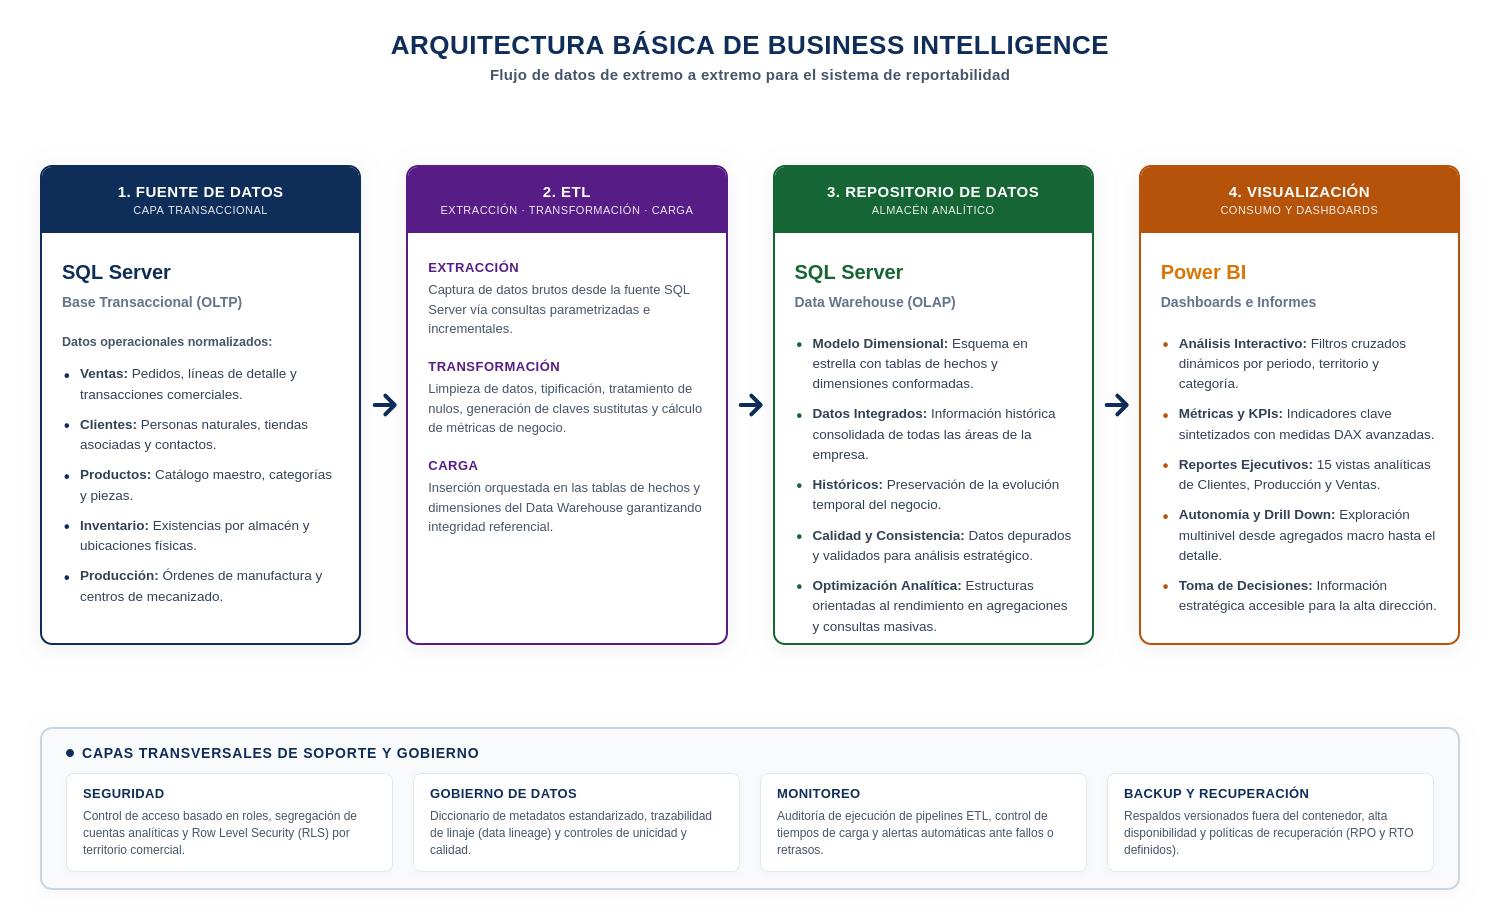
\includegraphics[width=0.85\textwidth]{figuras/arquitectura_propuesta.png}
    \caption{Arquitectura propuesta para la plataforma de reportabilidad.}
    \label{fig:arquitectura}
\end{figure}

\subsection{Capas del Flujo Principal}
\begin{enumerate}[leftmargin=*]
    \item \textbf{Fuente de Datos (OLTP):} Motor relacional \textit{Microsoft SQL Server 2022} ejecutado en contenedor Docker con la base transaccional \texttt{AdventureWorks2022}. Alberga las operaciones de ventas, catálogo de productos, órdenes de manufactura, clientes y personal.
    \item \textbf{Capa ETL (Extracción, Transformación y Carga):} Procesos de extracción desde la fuente relacional, limpieza y validación de atributos, aplicación de lógica de negocio y carga estructurada en el repositorio analítico. Su desarrollo operativo corresponde a la Entrega 2.
    \item \textbf{Repositorio de Datos (Data Warehouse):} Repositorio centralizado en SQL Server modelado bajo esquema dimensional (tablas de hechos y dimensiones conformadas). Almacena el histórico limpio y optimizado para consultas analíticas.
    \item \textbf{Visualización y Dashboards (Power BI):} Cuadros de mando ejecutivos interactivos conectados directamente al Data Warehouse en modo importación (motor en memoria VertiPaq) para consumo gerencial.
\end{enumerate}

\subsection{Justificación de Exclusión de Cubos Multidimensionales}
A diferencia del diagrama referencial preliminar de la cátedra, \textbf{se excluye la capa de cubos OLAP independientes} (SSAS multidimensional tradicional). Esta decisión simplifica la arquitectura sin perder capacidad analítica, ya que \textit{Power BI} incorpora de forma nativa un motor semántico columnar en memoria de alto rendimiento, reduciendo costos de mantenimiento, latencia de procesamiento y complejidad de infraestructura.

\subsection{Capas Transversales}
\begin{itemize}[leftmargin=*]
    \item \textbf{Seguridad:} Control de acceso basado en roles y proyección de seguridad a nivel de fila (\textit{Row Level Security} - RLS) según territorio comercial.
    \item \textbf{Gobierno de Datos:} Catálogo y diccionario de datos, trazabilidad de linaje (\textit{data lineage}) y reglas de consistencia.
    \item \textbf{Monitoreo:} Trazabilidad de ejecución de tareas ETL y alertas tempranas ante anomalías de carga.
    \item \textbf{Backup y Recuperación:} Respaldo periódico y políticas de recuperación ante contingencias de datos.
\end{itemize}

% ==============================================================================
% 2. BASE DE DATOS TRANSACCIONAL IMPLEMENTADA
% ==============================================================================
\section{Base de Datos Transaccional Implementada}

\subsection{Entorno y Puesta en Marcha en Docker}
Para garantizar portabilidad y reproducibilidad, la base de datos transaccional se implementó utilizando \textbf{Docker Desktop} mediante \textit{SQL Server 2022 Developer Edition}, configurando persistencia de datos en el volumen Docker \texttt{bigdata-sqlserver-data} y exponiendo el puerto estándar \texttt{1433}.

La base se restauró desde el respaldo oficial \texttt{AdventureWorks2022.bak}.

\subsection{Verificación de Esquemas y Registros}
La base cuenta con \textbf{71 tablas de usuario} agrupadas en 6 esquemas funcionales:
\begin{table}[H]
\centering
\small
\begin{tabular}{llr}
\toprule
\textbf{Esquema} & \textbf{Dominio Operacional} & \textbf{Tablas} \\
\midrule
\texttt{Production} & Fabricación, inventarios, productos y centros de trabajo & 25 \\
\texttt{Sales} & Clientes, pedidos, cuotas, territorios y promociones & 19 \\
\texttt{Person} & Personas naturales, contactos y direcciones & 13 \\
\texttt{HumanResources} & Empleados, departamentos y turnos de trabajo & 6 \\
\texttt{Purchasing} & Proveedores y órdenes de compra & 5 \\
\texttt{dbo} & Tablas del sistema y bitácoras & 3 \\
\midrule
\textbf{Total} & & \textbf{71} \\
\bottomrule
\end{tabular}
\caption{Distribución de tablas por esquema en AdventureWorks2022.}
\end{table}

Se auditó la volumetría de las tablas transaccionales y maestras principales:
\begin{itemize}[leftmargin=*]
    \item \texttt{Sales.SalesOrderDetail}: \textbf{121.317} líneas de detalle de venta.
    \item \texttt{Production.WorkOrder}: \textbf{72.591} órdenes de manufactura.
    \item \texttt{Sales.SalesOrderHeader}: \textbf{31.465} encabezados de órdenes de venta.
    \item \texttt{Person.Person}: \textbf{19.972} personas y contactos registrados.
    \item \texttt{Sales.Customer}: \textbf{19.820} cuentas de clientes habilitadas.
    \item \texttt{Production.ProductInventory}: \textbf{1.069} registros de existencias por ubicación.
    \item \texttt{Production.Product}: \textbf{504} productos en catálogo (295 terminados para venta).
\end{itemize}

\subsection{Evidencias de la Fuente de Datos}
En la Figura \ref{fig:ssms} se constata la conexión y despliegue de las tablas en \textit{SQL Server Management Studio} (SSMS), y en la Figura \ref{fig:modelo_relacional} se presenta el diagrama relacional simplificado de las entidades centrales.

\begin{figure}[H]
    \centering
    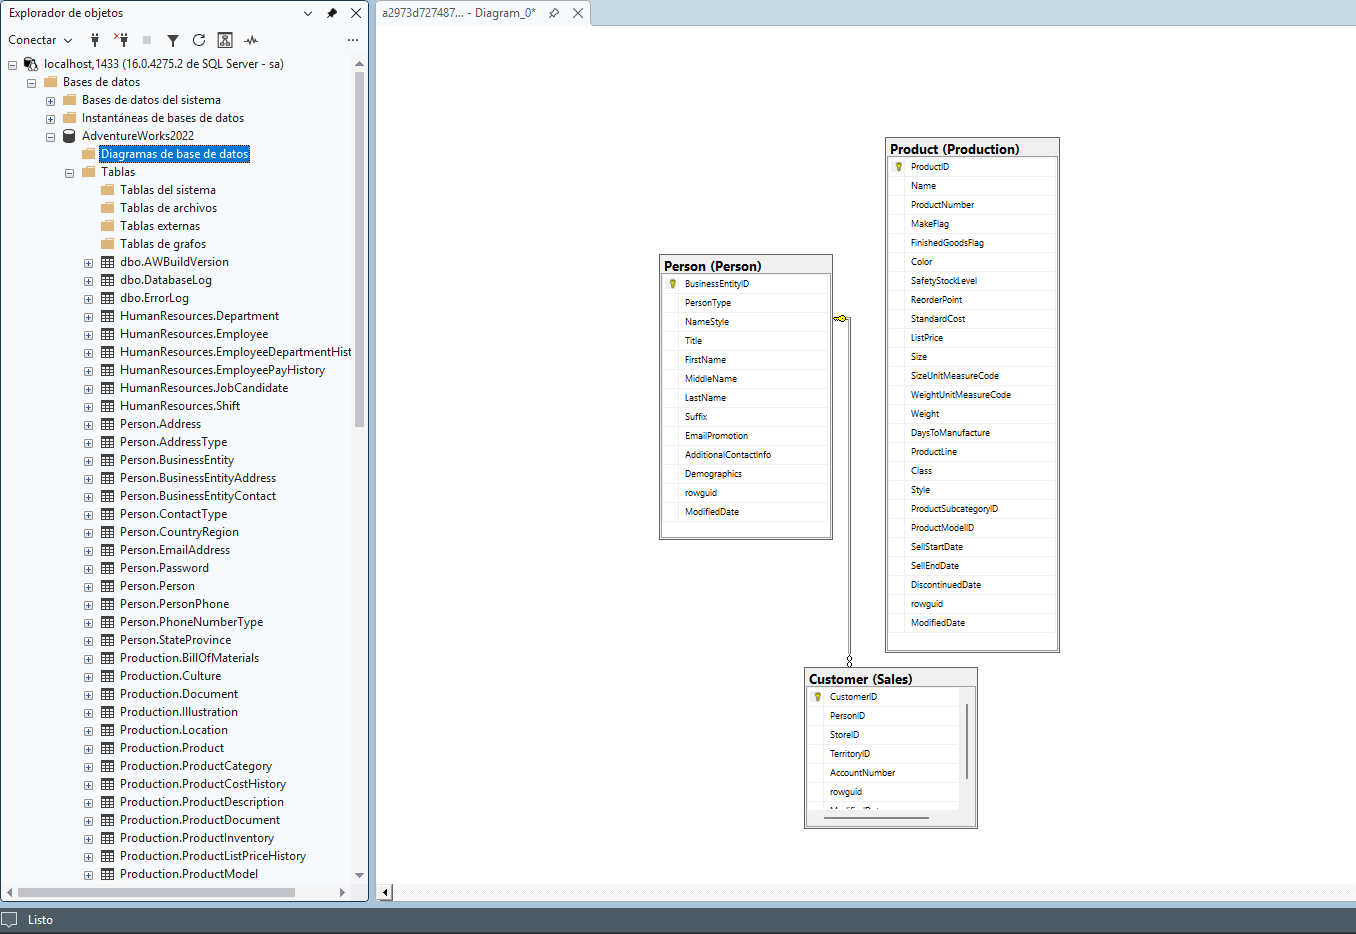
\includegraphics[width=0.68\textwidth]{figuras/ssms_tablas.png}
    \caption{Base de datos AdventureWorks2022 ONLINE verificada en SSMS.}
    \label{fig:ssms}
\end{figure}

\begin{figure}[H]
    \centering
    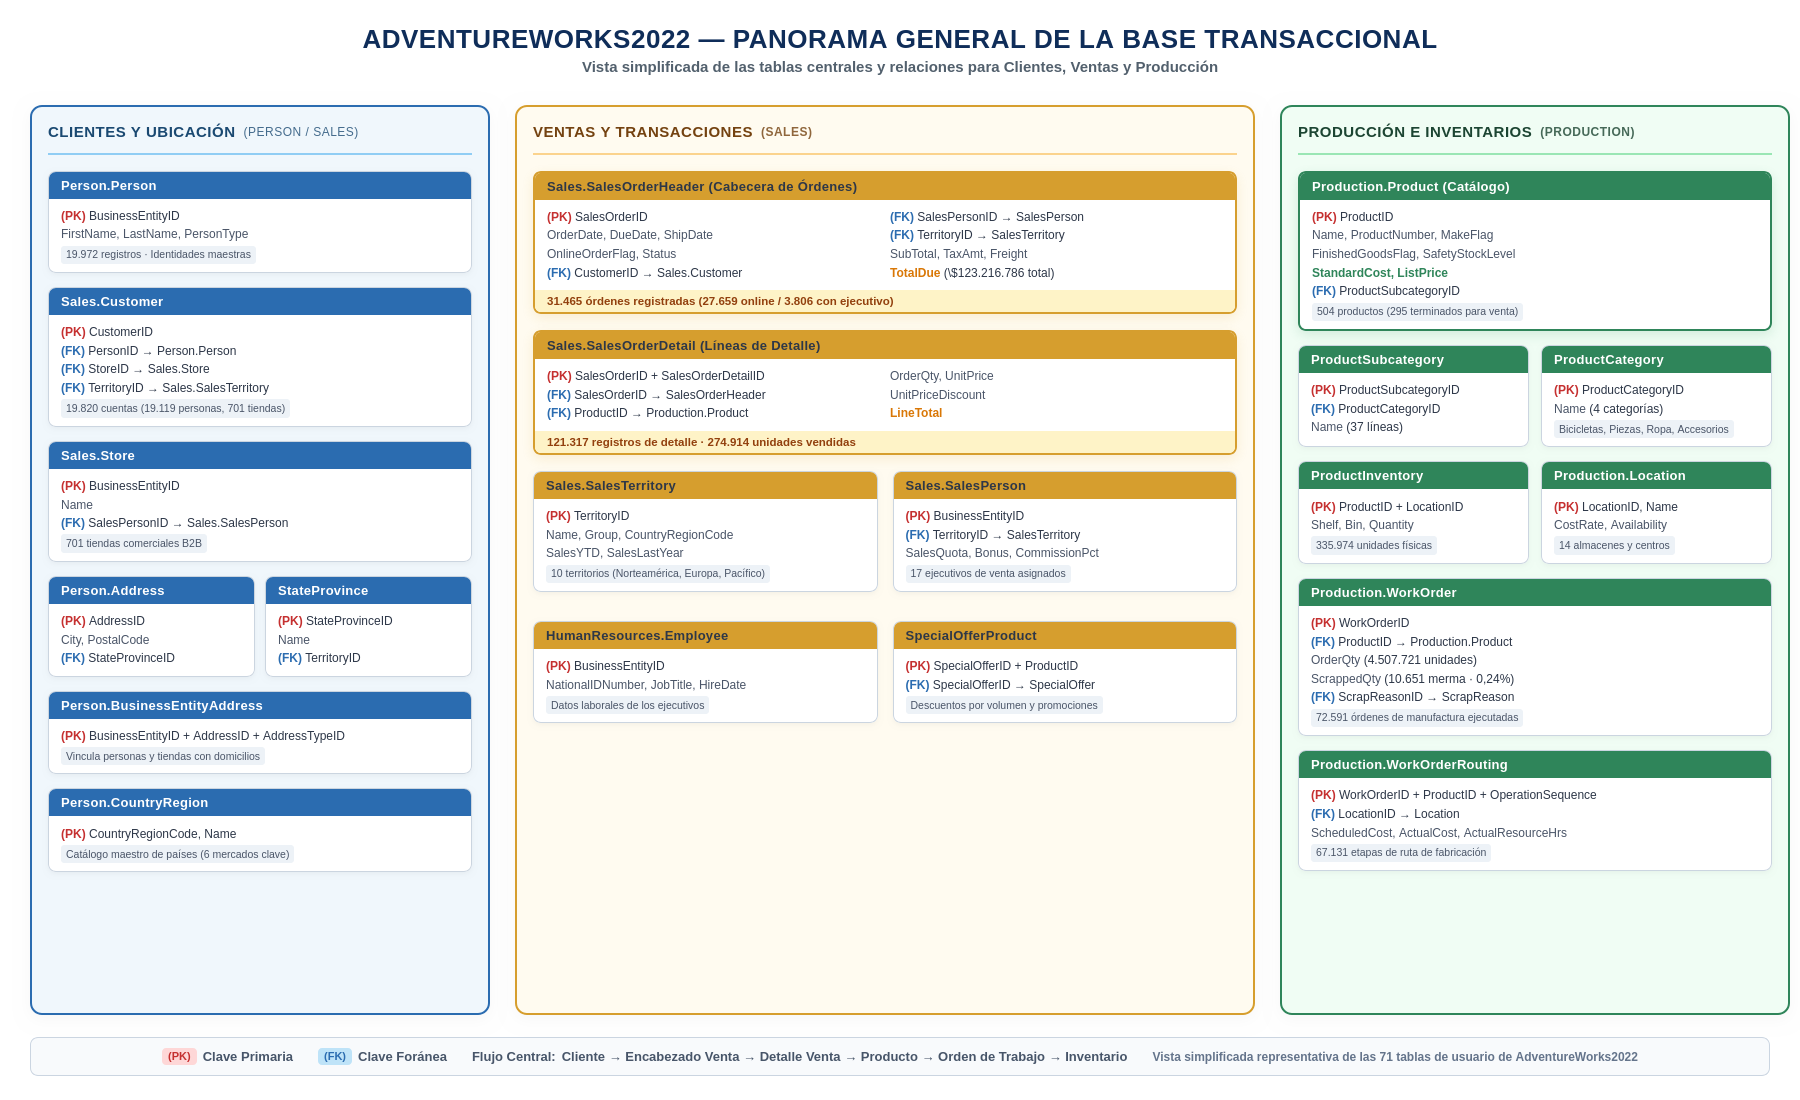
\includegraphics[width=0.80\textwidth]{figuras/modelo_relacional.png}
    \caption{Diagrama relacional simplificado de las entidades transaccionales centrales.}
    \label{fig:modelo_relacional}
\end{figure}

% ==============================================================================
% 3. DISEÑO DE LOS REPORTES SOLICITADOS
% ==============================================================================
\newpage
\section{Diseño de los Reportes Solicitados}

Se diseñaron \textbf{15 reportes analíticos} distribuidos equitativamente en tres perspectivas (5 reportes por perspectiva), verificando que cada indicador tenga respaldo directo en las tablas transaccionales de \textit{AdventureWorks2022}.

\subsection{Perspectiva 1: Clientes}
\begin{table}[H]
\centering
\small
\begin{tabularx}{\textwidth}{lp{3.2cm}p{4.2cm}Xp{2.8cm}}
\toprule
\textbf{Cód.} & \textbf{Reporte} & \textbf{Objetivo} & \textbf{KPIs Clave} & \textbf{Tablas Origen} \\
\midrule
\textbf{C1} & Panorama general & Composición de cartera individual vs tiendas y cobertura geográfica. & Clientes (19.820), con compras (19.119), individuales (96,5\,\%), tiendas (3,5\,\%). & \texttt{Sales.Customer}, \texttt{Person.Person}, \texttt{Sales.Store} \\
\addlinespace
\textbf{C2} & Valor y ranking & Identificar clientes de mayor facturación acumulada (Pareto). & Ventas acumuladas (\$123,2M), ticket promedio (\$3.916), órdenes/cliente (1,65). & \texttt{Sales.Customer}, \texttt{SalesOrderHeader} \\
\addlinespace
\textbf{C3} & Frecuencia y recencia & Segmentación según última compra y repetición de pedidos (RFM). & Clientes frecuentes (4.340), recurrentes (2.900), compra única (11.879), recencia (138 días). & \texttt{Sales.Customer}, \texttt{SalesOrderHeader} \\
\addlinespace
\textbf{C4} & Distribución geográfica & Concentración de clientes y venta promedio por territorio. & Territorios (10), países (6), mayor concentración Suroeste (4.696), venta/cliente (\$6.445). & \texttt{Sales.Customer}, \texttt{SalesTerritory}, \texttt{Person.Address} \\
\addlinespace
\textbf{C5} & Canal de compra & Comportamiento órdenes en línea (B2C) vs con vendedor (B2B). & Órdenes online (27.659; 87,9\,\%), vendedor (3.806; 12,1\,\%), ticket online (\$1.080) vs vendedor (\$24.530). & \texttt{SalesOrderHeader}, \texttt{Sales.Customer} \\
\bottomrule
\end{tabularx}
\caption{Ficha de diseño para la perspectiva de Clientes.}
\end{table}

\subsection{Perspectiva 2: Procesos y Producción}
\begin{table}[H]
\centering
\small
\begin{tabularx}{\textwidth}{lp{3.2cm}p{4.2cm}Xp{2.8cm}}
\toprule
\textbf{Cód.} & \textbf{Reporte} & \textbf{Objetivo} & \textbf{KPIs Clave} & \textbf{Tablas Origen} \\
\midrule
\textbf{P1} & Resumen general & Volumen físico planificado y evolución de órdenes de trabajo. & Órdenes trabajo (72.591), unidades planificadas (4.507.721), desechadas (10.651), merma (0,24\,\%). & \texttt{Production.WorkOrder}, \texttt{Production.Product} \\
\addlinespace
\textbf{P2} & Calidad y desperdicio & Causas y productos con mayor tasa de descarte (\textit{scrap}). & Unidades desechadas (10.651), tasa desperdicio (0,24\,\%), motivos registrados (16), órdenes con descarte (2.840). & \texttt{Production.WorkOrder}, \texttt{ScrapReason} \\
\addlinespace
\textbf{P3} & Inventario y stock & Control de existencias por ubicación física y alertas de reposición. & Unidades disponibles (335.974), productos con stock (432), ubicaciones (14), bajo reorden (68). & \texttt{ProductInventory}, \texttt{Location}, \texttt{Product} \\
\addlinespace
\textbf{P4} & Rendimiento operacional & Desviación de horas y costos reales vs planificados por centro. & Operaciones (67.131), horas reales (228.962), costo planificado (\$3,48M), costo real (\$3,48M). & \texttt{WorkOrderRouting}, \texttt{Production.Location} \\
\addlinespace
\textbf{P5} & Portafolio de productos & Composición del catálogo, fabricación interna, costos y precios. & Productos catálogo (504), terminados (295), categorías (4), subcategorías (37). & \texttt{Product}, \texttt{ProductCategory}, \texttt{ProductSubcategory} \\
\bottomrule
\end{tabularx}
\caption{Ficha de diseño para la perspectiva de Procesos y Producción.}
\end{table}

\subsection{Perspectiva 3: Ventas}
\begin{table}[H]
\centering
\small
\begin{tabularx}{\textwidth}{lp{3.2cm}p{4.2cm}Xp{2.8cm}}
\toprule
\textbf{Cód.} & \textbf{Reporte} & \textbf{Objetivo} & \textbf{KPIs Clave} & \textbf{Tablas Origen} \\
\midrule
\textbf{V1} & Resumen ejecutivo & Salud comercial global, ingresos consolidados y evolución mensual. & Ventas totales (\$123.216.786), órdenes (31.465), unidades vendidas (274.914), ticket (\$3.916). & \texttt{SalesOrderHeader}, \texttt{SalesOrderDetail} \\
\addlinespace
\textbf{V2} & Productos y categorías & Ventas y rentabilidad por línea de producto y categoría. & Productos con venta (266), unidades vendidas (274.914), categorías (4), precio promedio (\$425). & \texttt{SalesOrderDetail}, \texttt{Product}, \texttt{ProductCategory} \\
\addlinespace
\textbf{V3} & Territorios & Desempeño regional y participación nacional vs internacional. & Territorios activos (10), ventas (\$123,2M), venta internacional (44,8\,\%), ticket territorial (\$3.916). & \texttt{SalesOrderHeader}, \texttt{SalesTerritory} \\
\addlinespace
\textbf{V4} & Vendedores & Cumplimiento de cuotas comerciales de ejecutivos presenciales. & Vendedores (17), órdenes asistidas (3.806), ventas (\$93,39M), cumplimiento cuota (104,2\,\%). & \texttt{SalesPerson}, \texttt{SalesOrderHeader}, \texttt{Person.Person} \\
\addlinespace
\textbf{V5} & Descuentos y ofertas & Impacto de descuentos por volumen y promociones en la venta neta. & Venta bruta (\$126,4M), descuentos (\$3,18M), venta neta (\$123,2M), descuento medio (2,52\,\%). & \texttt{SalesOrderDetail}, \texttt{SpecialOffer}, \texttt{SalesOrderHeader} \\
\bottomrule
\end{tabularx}
\caption{Ficha de diseño para la perspectiva de Ventas.}
\end{table}

% ------------------------------------------------------------------------------
% 3.4 TODOS LOS 15 MOCKUPS INTERACTIVOS
% ------------------------------------------------------------------------------
\subsection{Validación Temprana mediante los 15 Mockups Interactivos}
Para comprobar anticipadamente la viabilidad y experiencia visual previa a Power BI, se implementó una aplicación web interactiva en \texttt{Taller1/mocks/index.html} que incorpora los 15 reportes funcionales con reactividad a filtros de periodo (2011--2014) y territorio.

A continuación se presentan las 15 vistas conceptuales completas organizadas por perspectiva:

\subsubsection{Vistas de la Perspectiva de Clientes (C1 a C5)}

\begin{figure}[H]
    \centering
    \begin{subfigure}[b]{0.48\textwidth}
        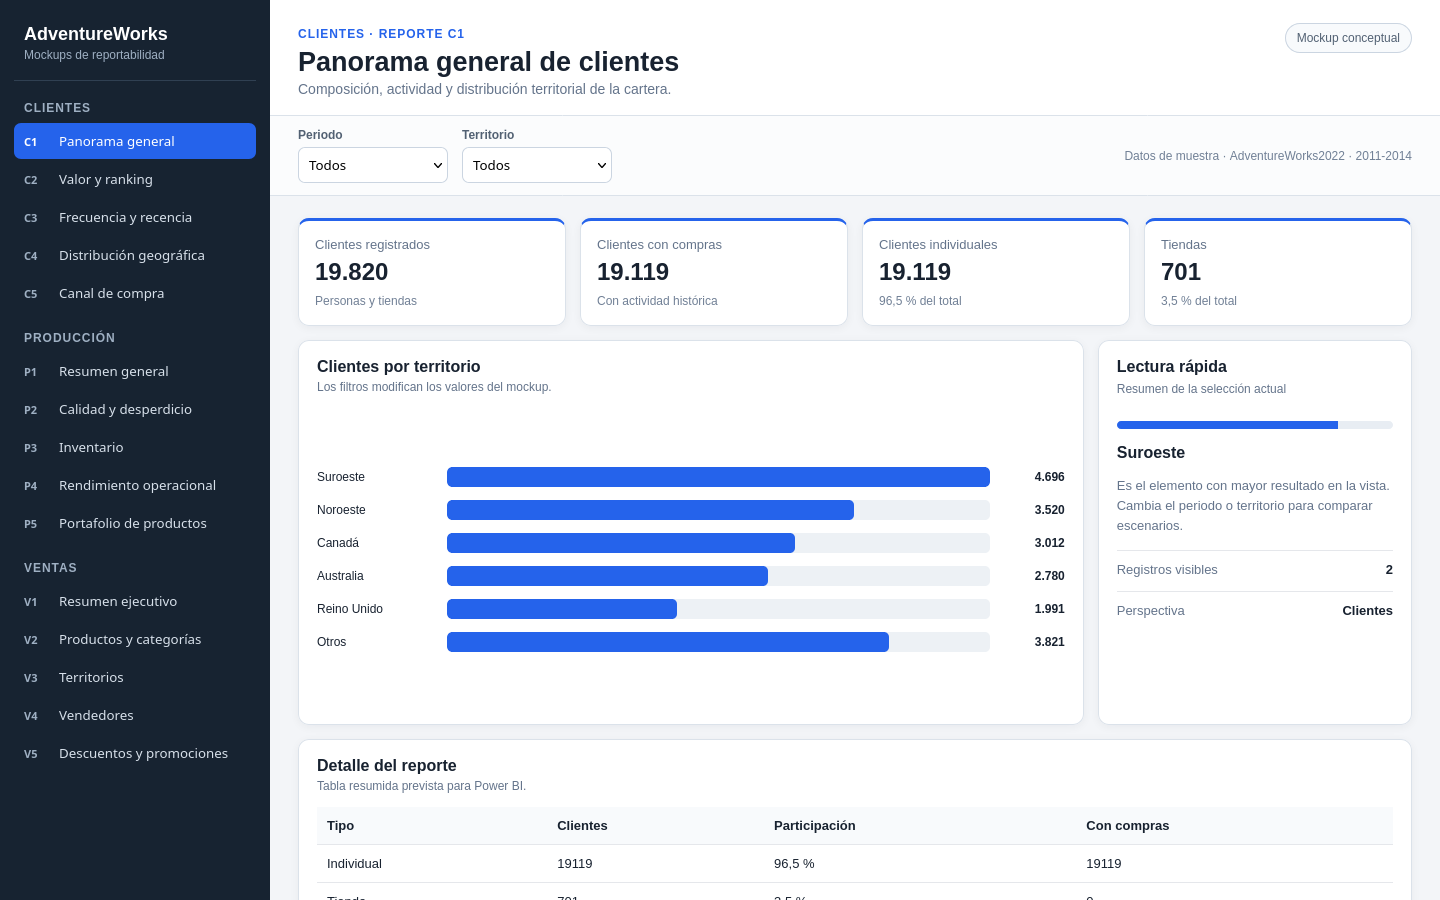
\includegraphics[width=\textwidth]{figuras/mockup_c1.png}
        \caption{C1: Panorama general de clientes.}
    \end{subfigure}
    \hfill
    \begin{subfigure}[b]{0.48\textwidth}
        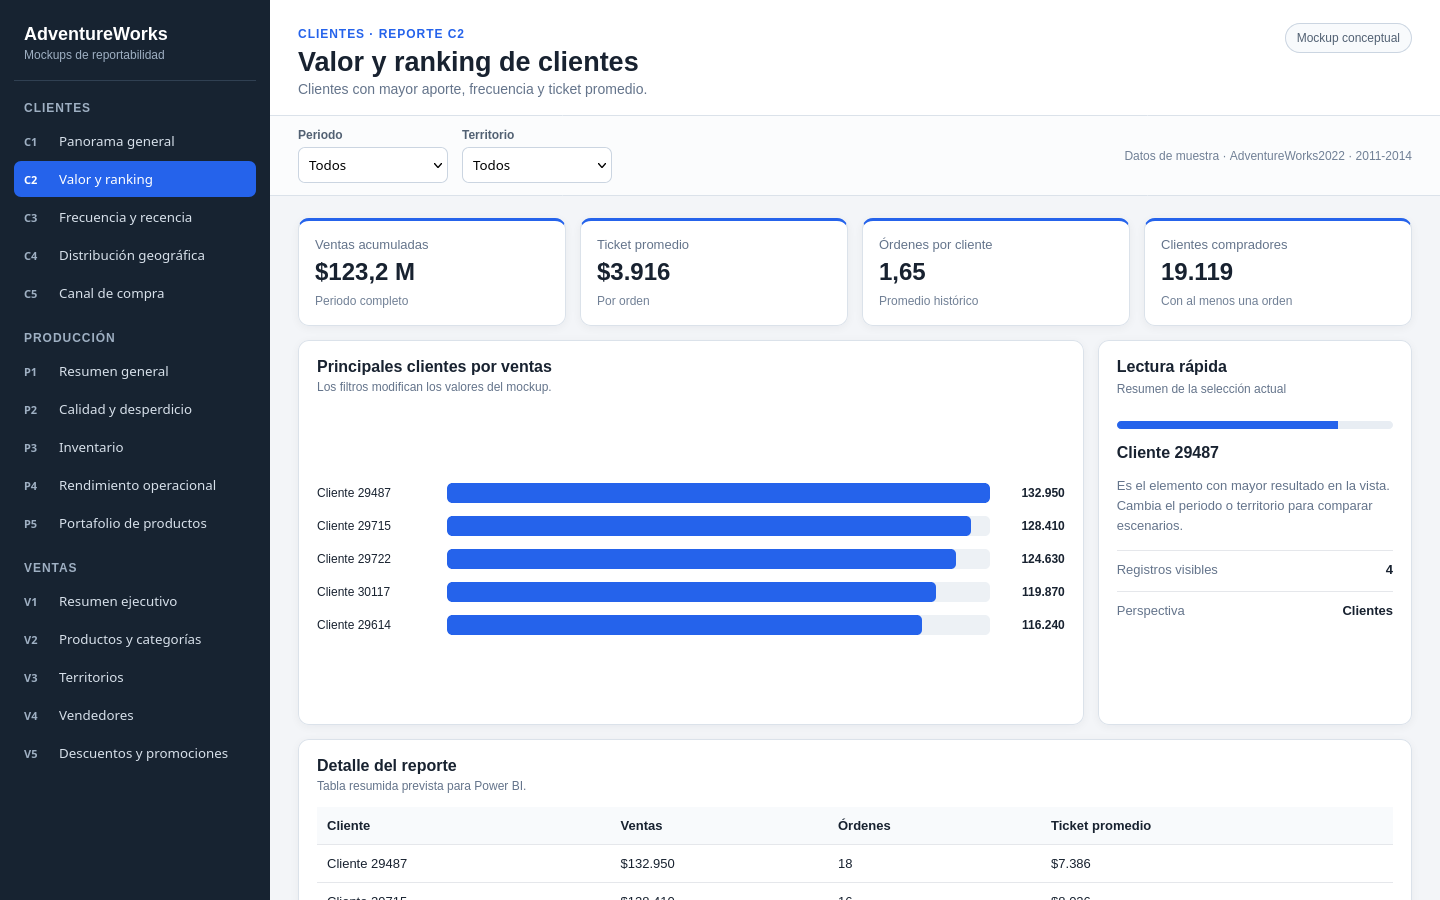
\includegraphics[width=\textwidth]{figuras/mockup_c2.png}
        \caption{C2: Valor y ranking de clientes.}
    \end{subfigure}
    \\[0.25cm]
    \begin{subfigure}[b]{0.48\textwidth}
        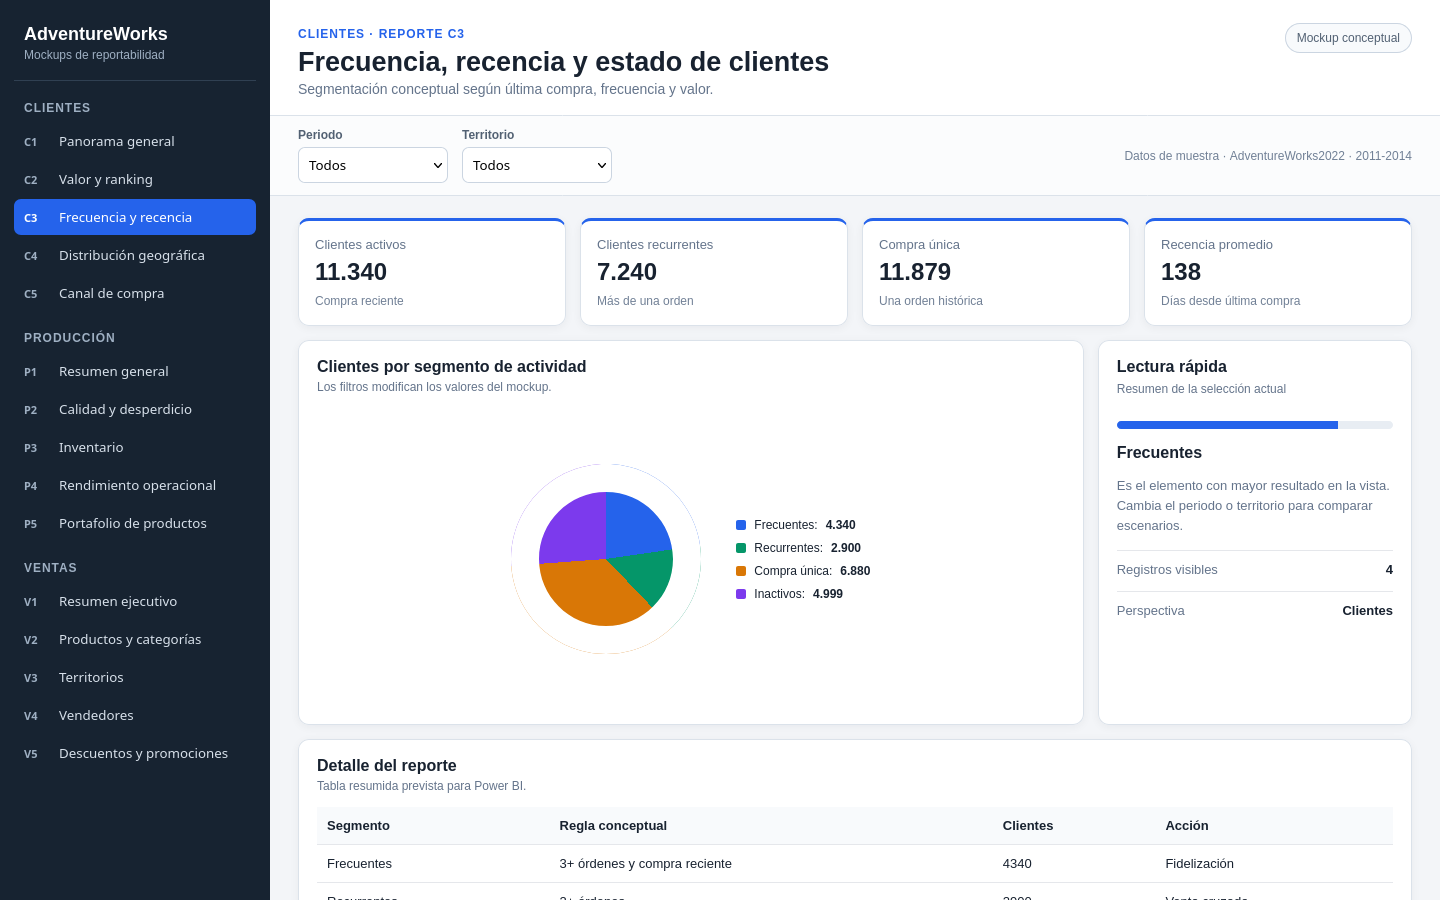
\includegraphics[width=\textwidth]{figuras/mockup_c3.png}
        \caption{C3: Frecuencia y recencia (RFM).}
    \end{subfigure}
    \hfill
    \begin{subfigure}[b]{0.48\textwidth}
        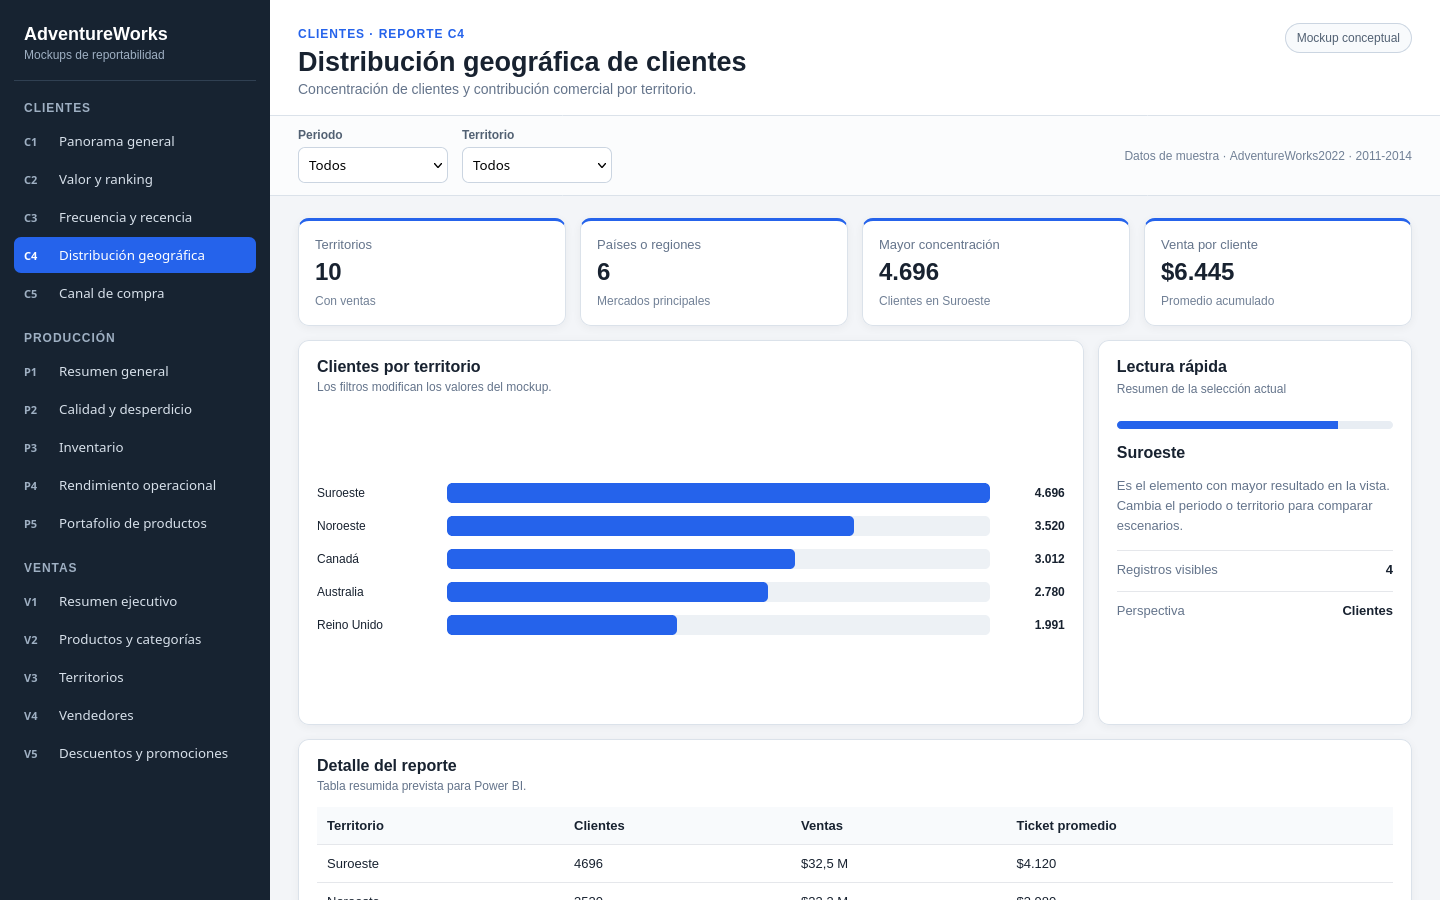
\includegraphics[width=\textwidth]{figuras/mockup_c4.png}
        \caption{C4: Distribución geográfica.}
    \end{subfigure}
    \\[0.25cm]
    \begin{subfigure}[b]{0.48\textwidth}
        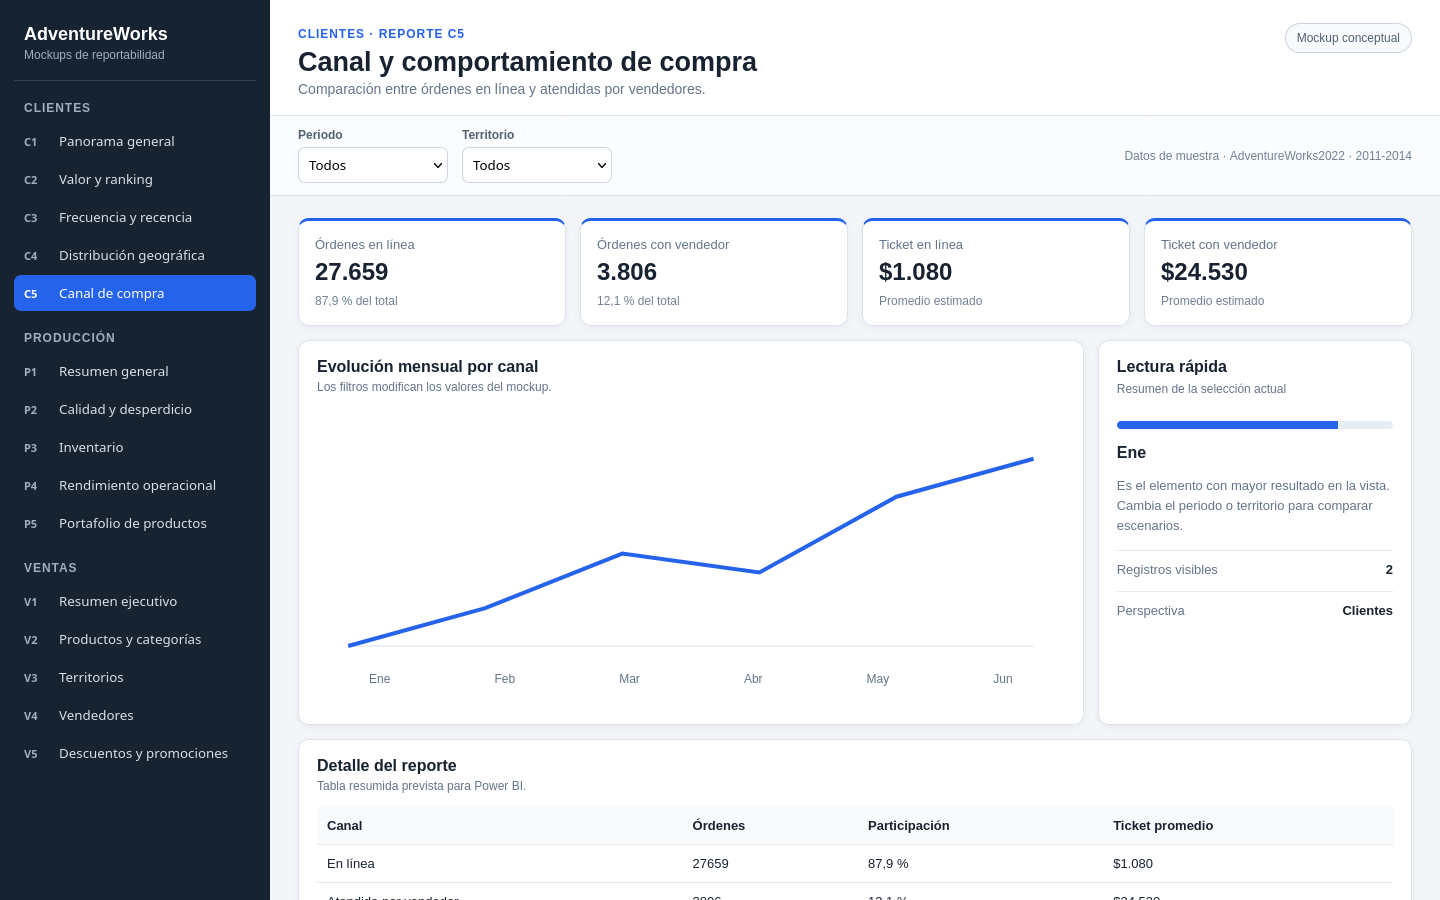
\includegraphics[width=\textwidth]{figuras/mockup_c5.png}
        \caption{C5: Canal de compra (Online vs Vendedor).}
    \end{subfigure}
    \caption{Mockups conceptuales para la perspectiva de Clientes (C1 a C5).}
    \label{fig:mockups_clientes}
\end{figure}

\newpage
\subsubsection{Vistas de la Perspectiva de Procesos y Producción (P1 a P5)}

\begin{figure}[H]
    \centering
    \begin{subfigure}[b]{0.48\textwidth}
        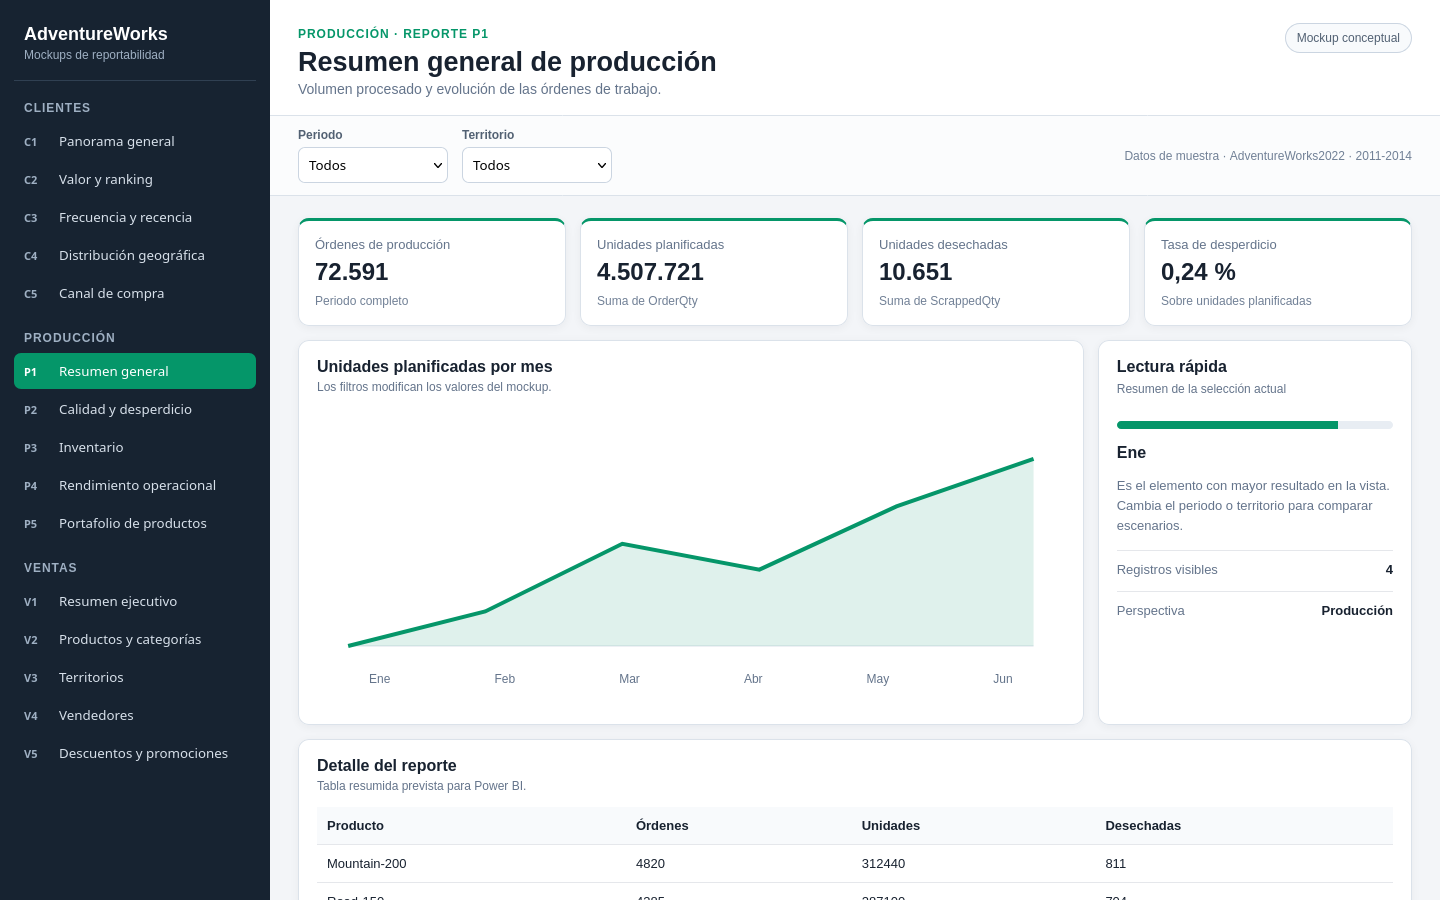
\includegraphics[width=\textwidth]{figuras/mockup_p1.png}
        \caption{P1: Resumen general de producción.}
    \end{subfigure}
    \hfill
    \begin{subfigure}[b]{0.48\textwidth}
        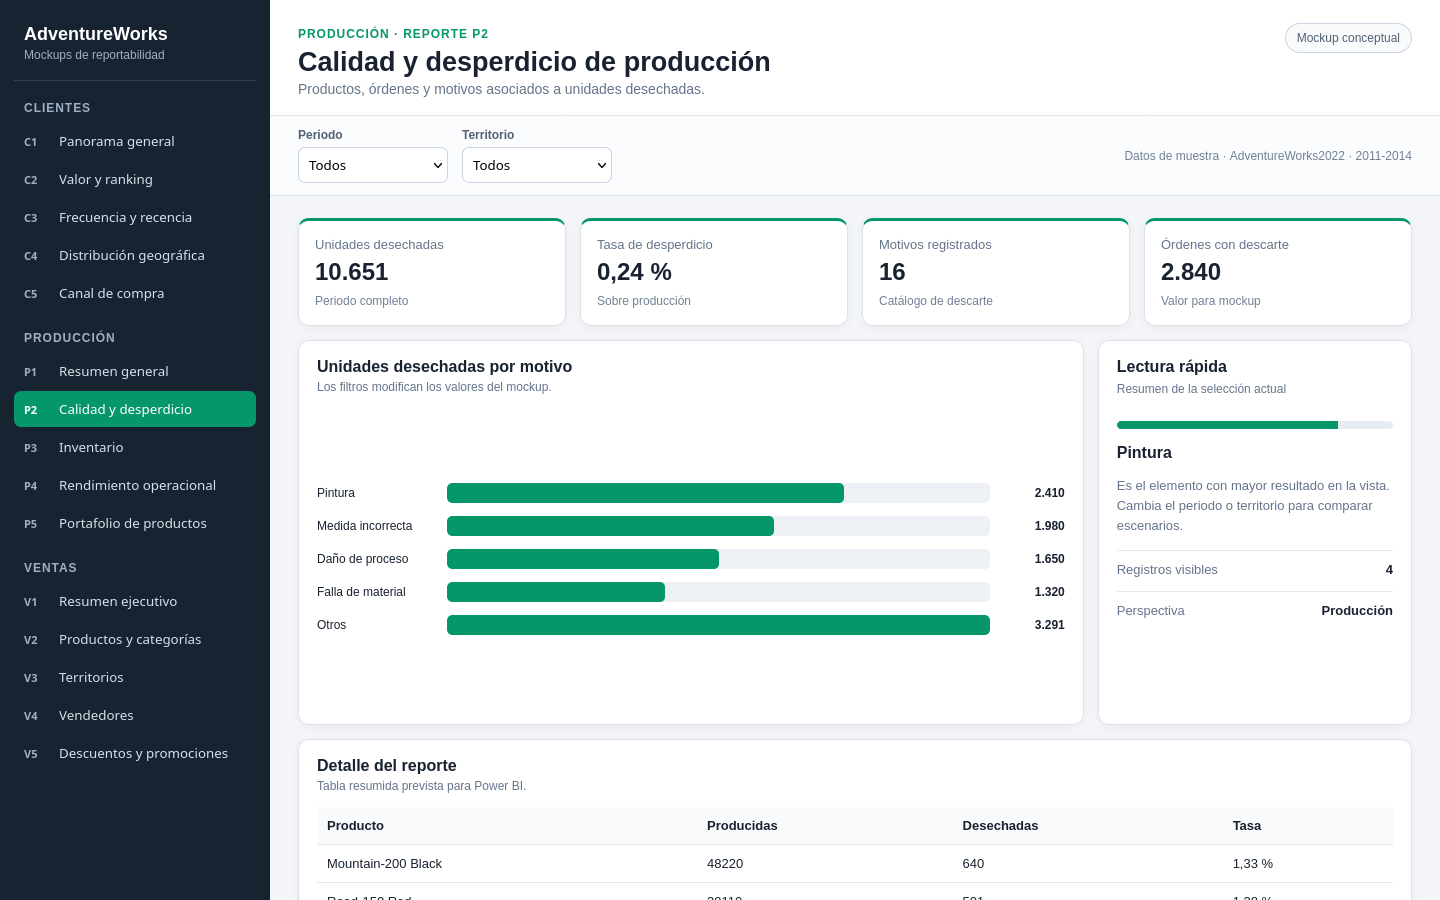
\includegraphics[width=\textwidth]{figuras/mockup_p2.png}
        \caption{P2: Calidad y desperdicio (Scrap).}
    \end{subfigure}
    \\[0.25cm]
    \begin{subfigure}[b]{0.48\textwidth}
        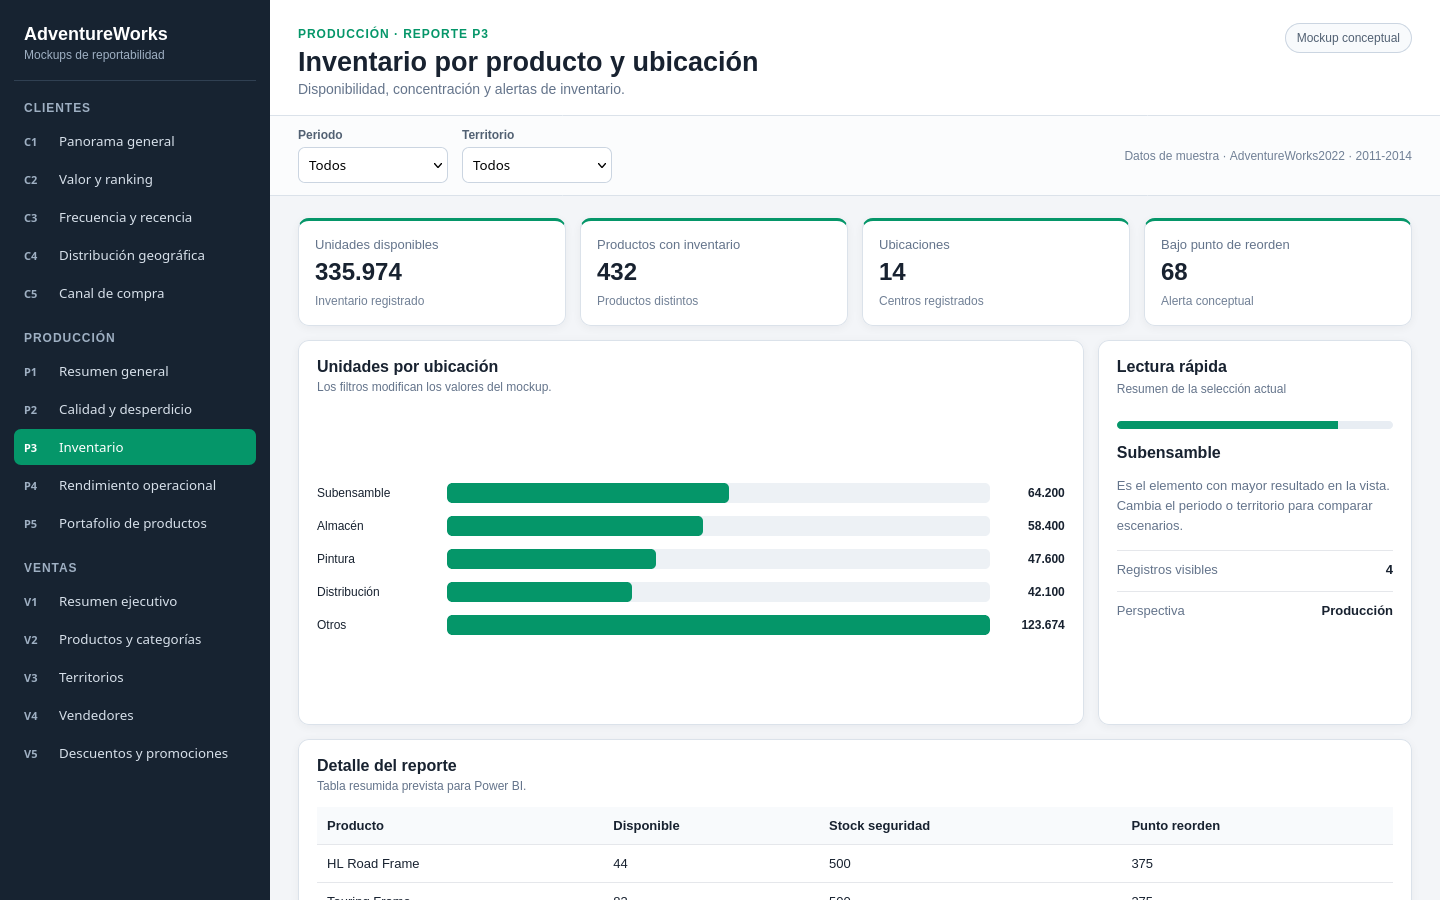
\includegraphics[width=\textwidth]{figuras/mockup_p3.png}
        \caption{P3: Inventario y existencias en almacén.}
    \end{subfigure}
    \hfill
    \begin{subfigure}[b]{0.48\textwidth}
        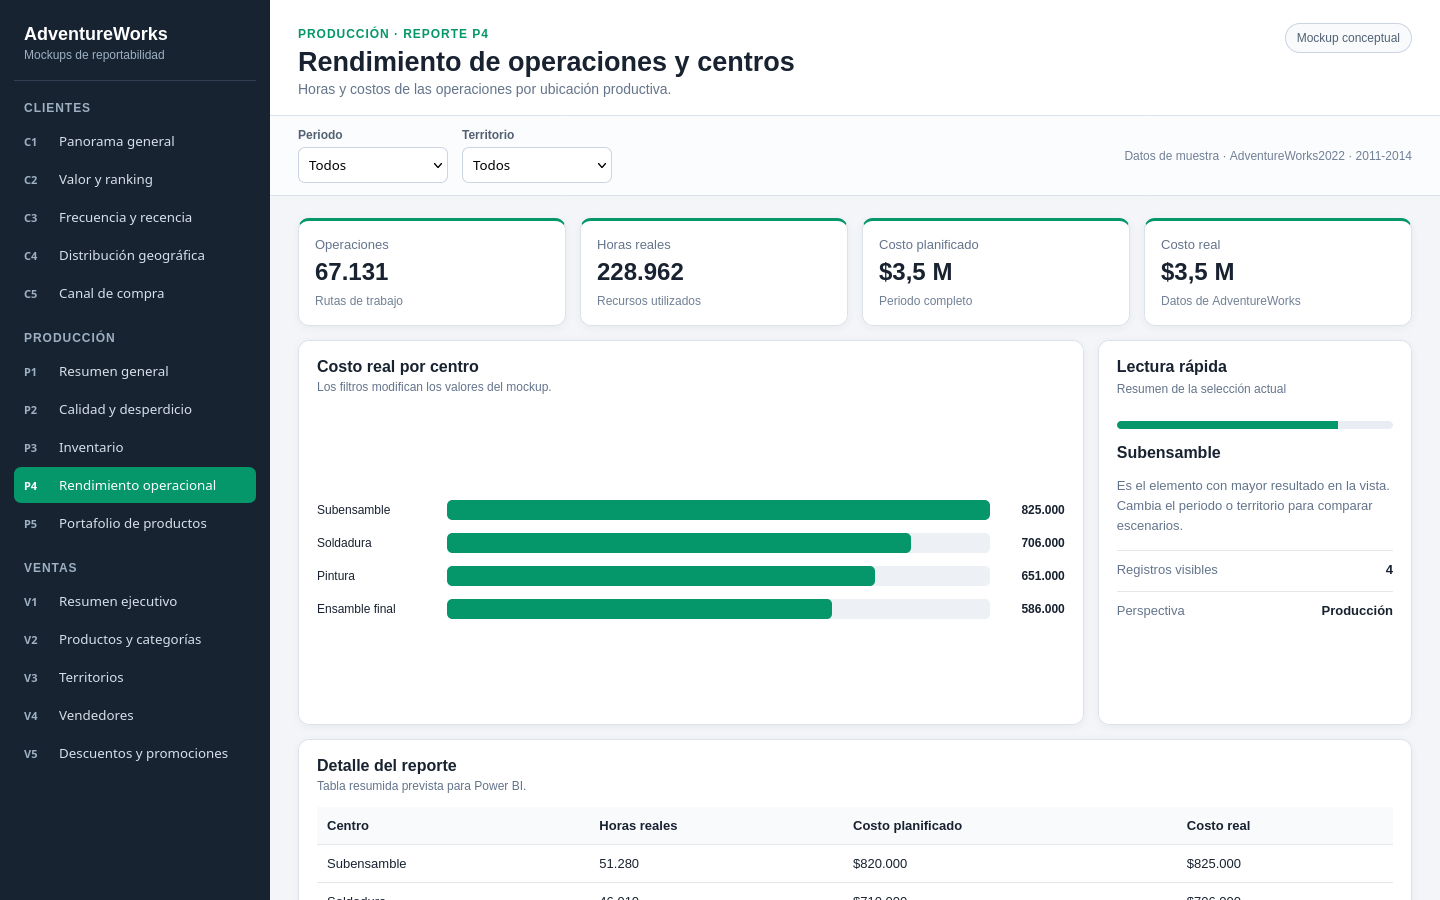
\includegraphics[width=\textwidth]{figuras/mockup_p4.png}
        \caption{P4: Rendimiento de centros operacionales.}
    \end{subfigure}
    \\[0.25cm]
    \begin{subfigure}[b]{0.48\textwidth}
        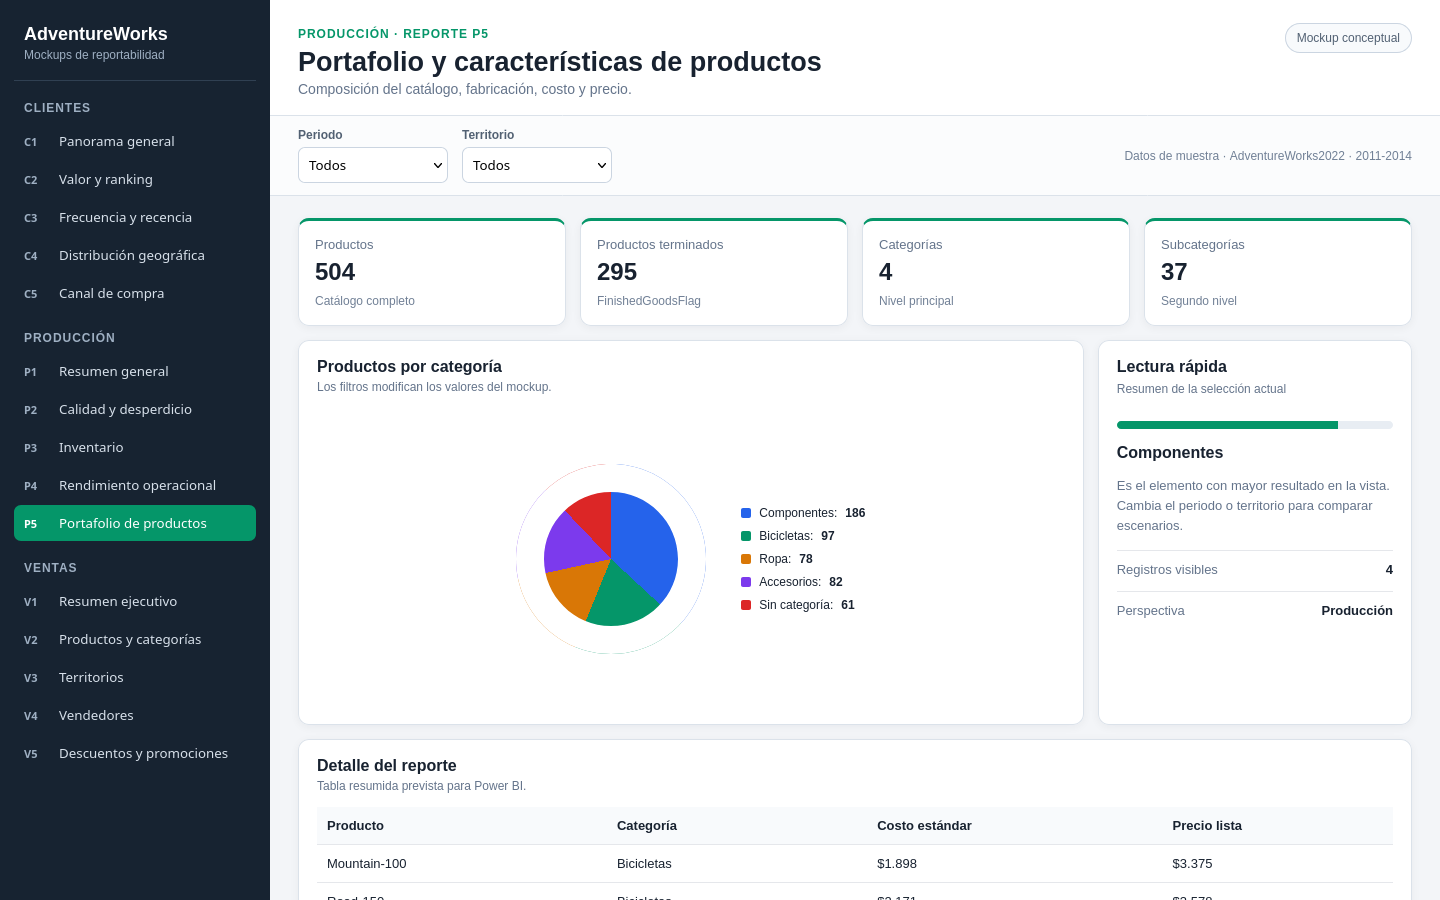
\includegraphics[width=\textwidth]{figuras/mockup_p5.png}
        \caption{P5: Portafolio y catálogo de productos.}
    \end{subfigure}
    \caption{Mockups conceptuales para la perspectiva de Procesos y Producción (P1 a P5).}
    \label{fig:mockups_produccion}
\end{figure}

\newpage
\subsubsection{Vistas de la Perspectiva de Ventas (V1 a V5)}

\begin{figure}[H]
    \centering
    \begin{subfigure}[b]{0.48\textwidth}
        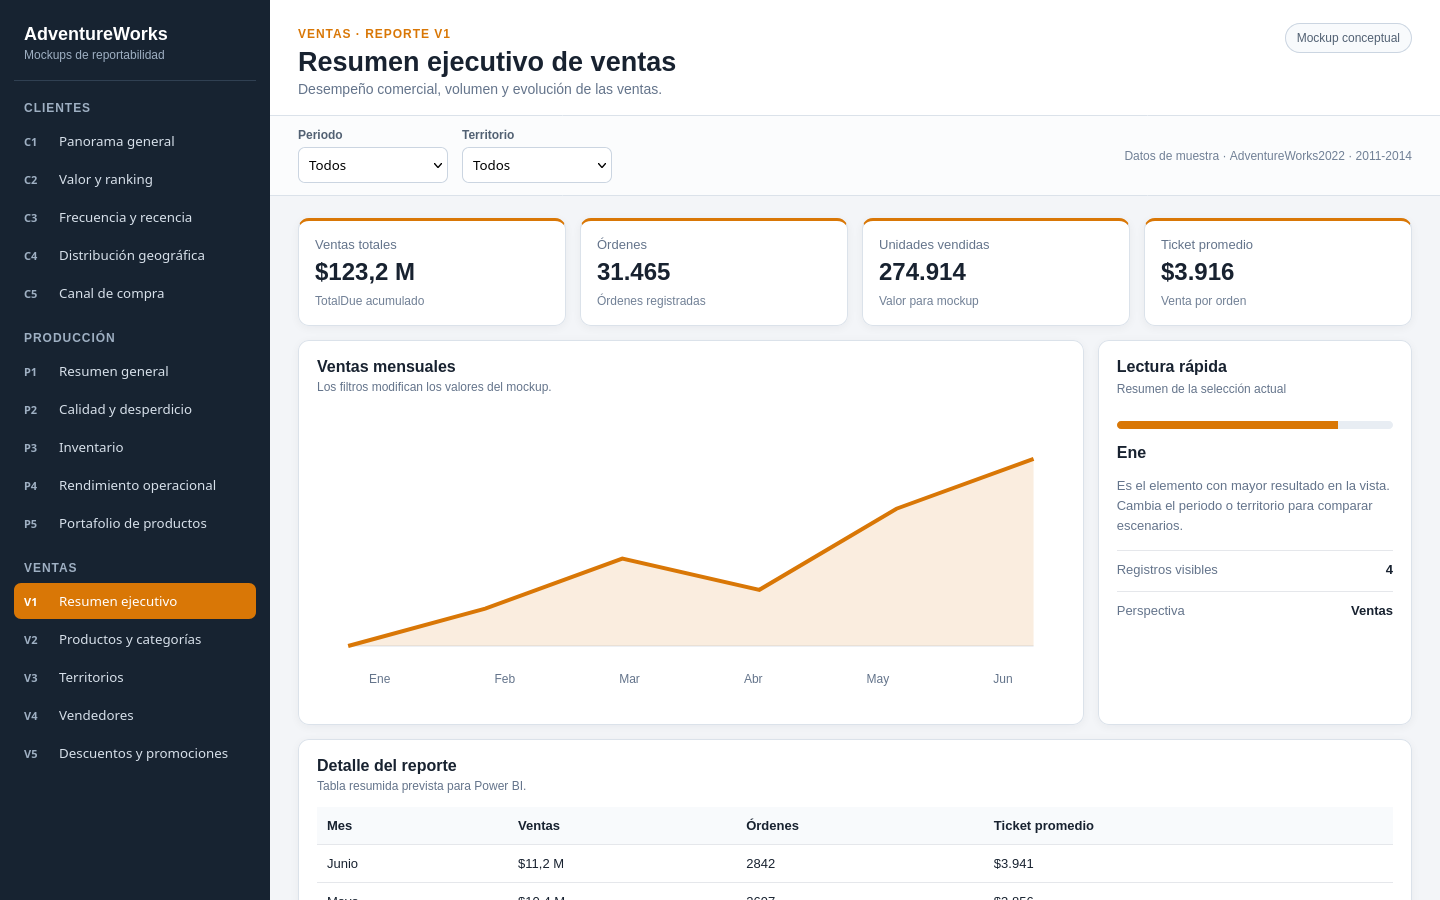
\includegraphics[width=\textwidth]{figuras/mockup_v1.png}
        \caption{V1: Resumen ejecutivo de ventas.}
    \end{subfigure}
    \hfill
    \begin{subfigure}[b]{0.48\textwidth}
        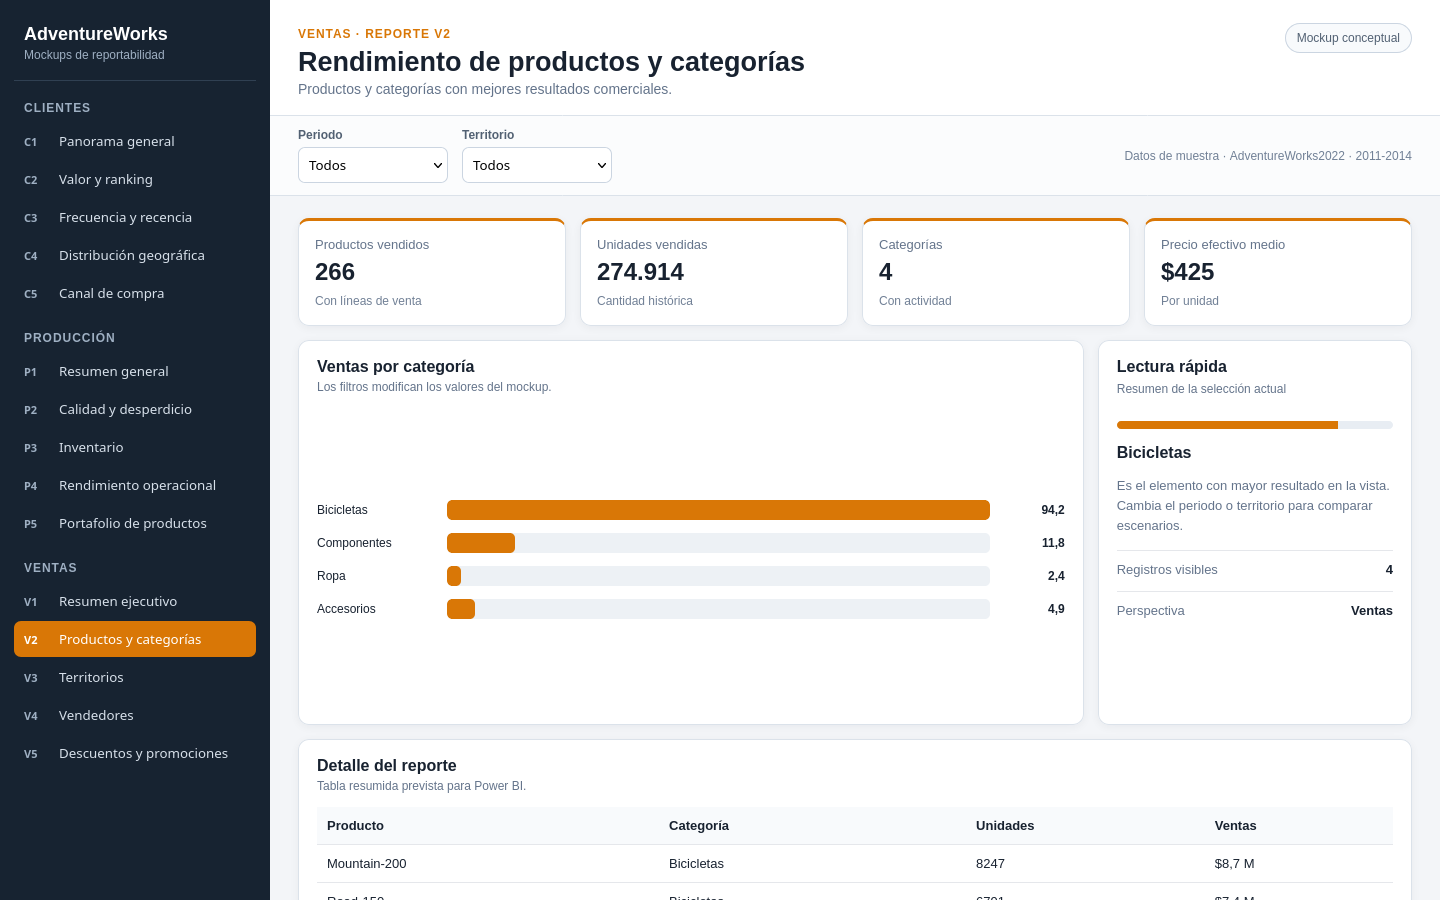
\includegraphics[width=\textwidth]{figuras/mockup_v2.png}
        \caption{V2: Rendimiento de productos y categorías.}
    \end{subfigure}
    \\[0.25cm]
    \begin{subfigure}[b]{0.48\textwidth}
        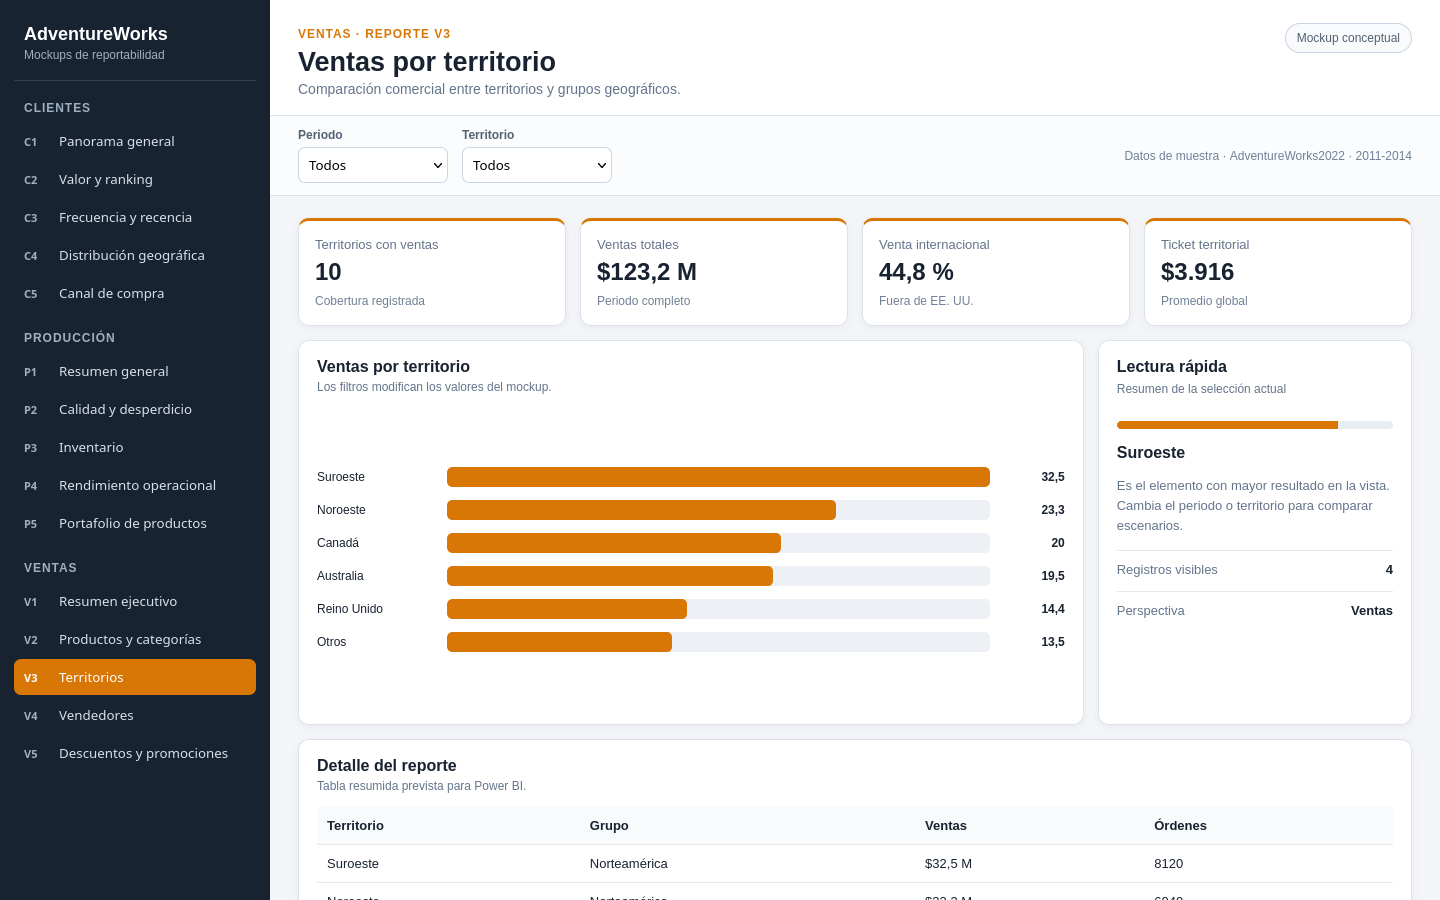
\includegraphics[width=\textwidth]{figuras/mockup_v3.png}
        \caption{V3: Ventas por territorio regional.}
    \end{subfigure}
    \hfill
    \begin{subfigure}[b]{0.48\textwidth}
        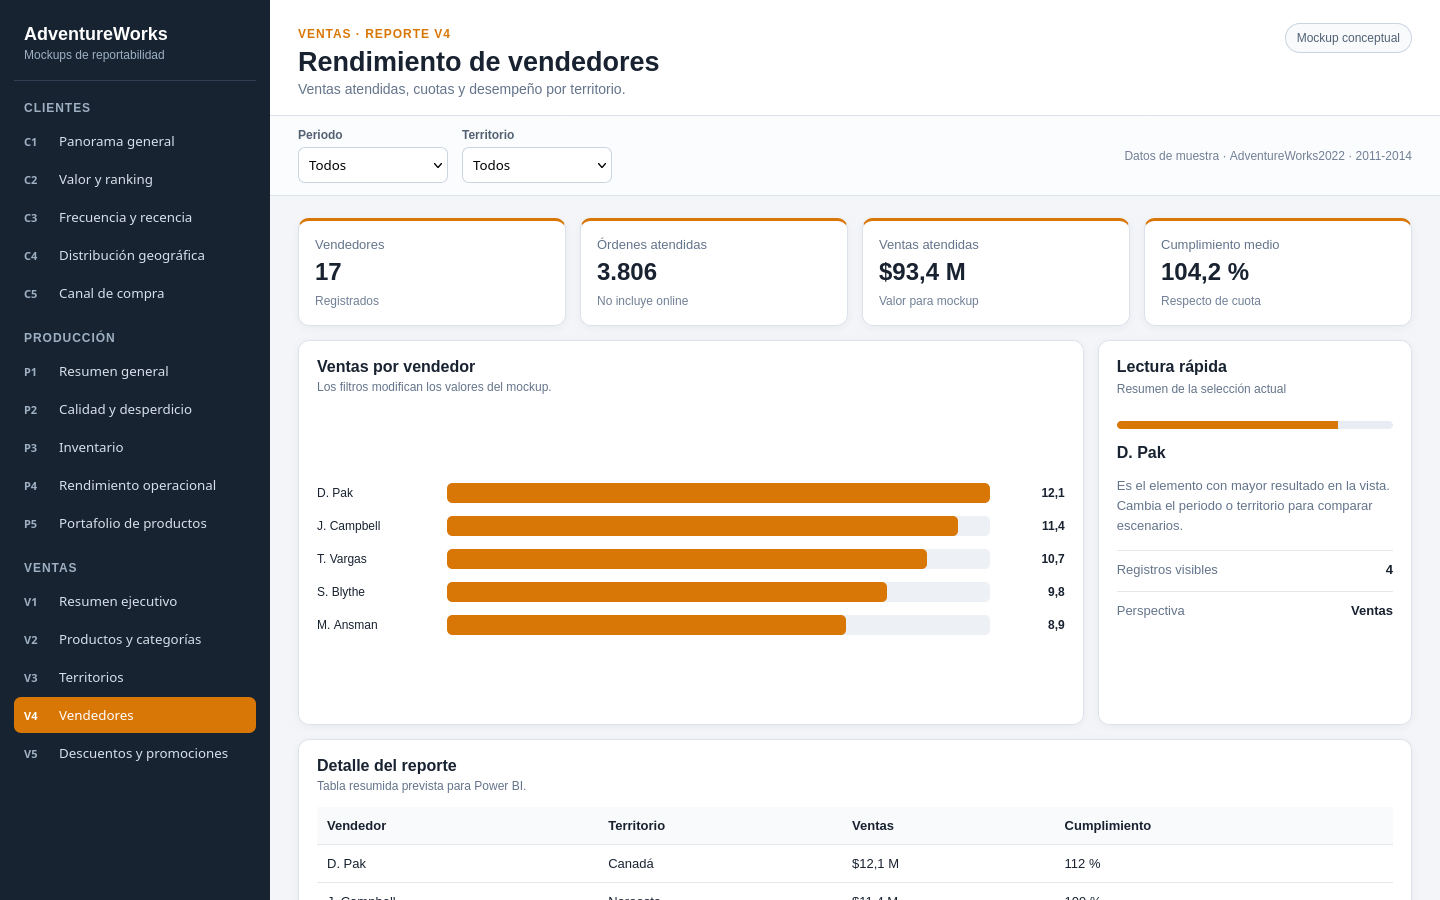
\includegraphics[width=\textwidth]{figuras/mockup_v4.png}
        \caption{V4: Desempeño y cuotas de vendedores.}
    \end{subfigure}
    \\[0.25cm]
    \begin{subfigure}[b]{0.48\textwidth}
        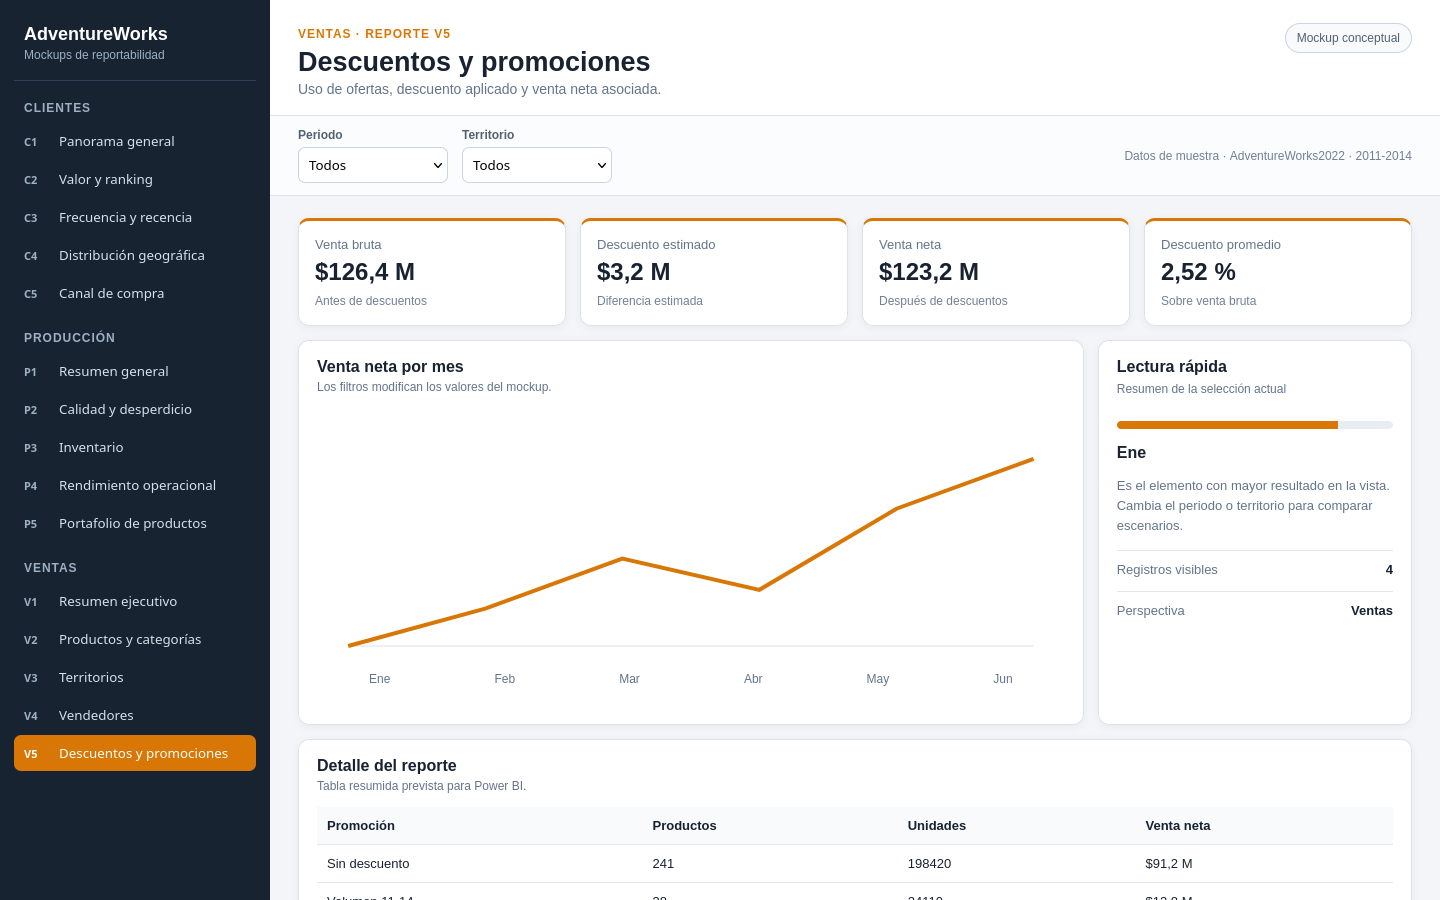
\includegraphics[width=\textwidth]{figuras/mockup_v5.png}
        \caption{V5: Descuentos, ofertas y venta neta.}
    \end{subfigure}
    \caption{Mockups conceptuales para la perspectiva de Ventas (V1 a V5).}
    \label{fig:mockups_ventas}
\end{figure}

% ==============================================================================
% 4. RESUMEN DE ENTREGABLES DEL PROYECTO
% ==============================================================================
\newpage
\section{Resumen de Entregables del Proyecto}

En conformidad con las pautas oficiales del curso para la \textbf{Entrega 1}, el entregable formal se consolida de la siguiente manera:

\begin{enumerate}[leftmargin=*]
    \item \textbf{Informe Técnico Oficial (este documento en PDF):}
    \begin{itemize}
        \item Diseño de la arquitectura de la solución (flujo de 4 capas desacopladas y capas transversales).
        \item Base de datos transaccional (fuente de datos) implementada y verificada en estado \texttt{ONLINE} con sus 71 tablas y volumetría operacional.
        \item Diseño conceptual y validación de los 15 reportes solicitados en las tres perspectivas de negocio requeridas (Clientes, Procesos y Ventas).
    \end{itemize}
\end{enumerate}

Para mayor detalle y verificación del entorno reproducible (configuración Docker, script de restauración de la base de datos, código fuente de los 15 mockups interactivos navegables y diagramas técnicos editables \texttt{.drawio}), adjuntamos el enlace oficial del repositorio del proyecto:

\begin{center}
    \url{https://github.com/Menderin/Ing.-de-Datos-y-Big-Data}
\end{center}

\end{document}
